\section{Zjednodušení schématu}
Zapojení s mikrokontrolerem ESP32 bylo poměrně komplexní. Po bližším ohledání produktů Espressif bylo zjištěno, že nabízejí alternativu pro ESP32 s více piny, integrovaným USB převodníkem, AI akcelerací a spoustou dalších funkcí.
\subsection{Porovnání ESP32 a ESP32-S3}
Jaké jsou tedy nejzásadnější rozdíly mezi mikrokontrolery ESP32 a ESP32-S3?

\begin{table}[htbp!]
	\centering
	\begin{tabularx}{\textwidth}{|X|X|X|}\hline
		ESP čip                  & ESP32     & ESP32 S3  \\ \hline
		počet jader              & 2         & 2         \\ \hline
		max. velikost \ac{FLASH} & 16MB      & 16MB      \\ \hline
		max. velikost \ac{psram} & NE        & 8MB       \\ \hline
		AI akcelerace            & NE        & ANO       \\ \hline
		počet GPIO               & 24        & 36        \\ \hline
		usb převodník            & NE        & ANO       \\ \hline
		cena za modul            & cca 100kč & cca 120kč \\ \hline
	\end{tabularx}
	\label{tab:Tabulka_porovnani_ESP_ESP_S3}
	\caption{Tabulka porovnání ESP32 a ESP32 S3}
	\cite{ESP32_datasheet}
	\cite{ESP32_S3_datasheet}
	\cite{esp32-module_schematics}
	\cite{ESP32-S3-module_schematics}
	\cite{espressif}
\end{table}



\subsection{Popis schémat mk.II}
Následující podkapiitoly se budou zabývat popisem rozdílů mezí 1. a 2. verzí schémat.

\subsection{Celek}
Opět popisuje provázanost mezi schématy. UART vyměněn za USB.
\newpage
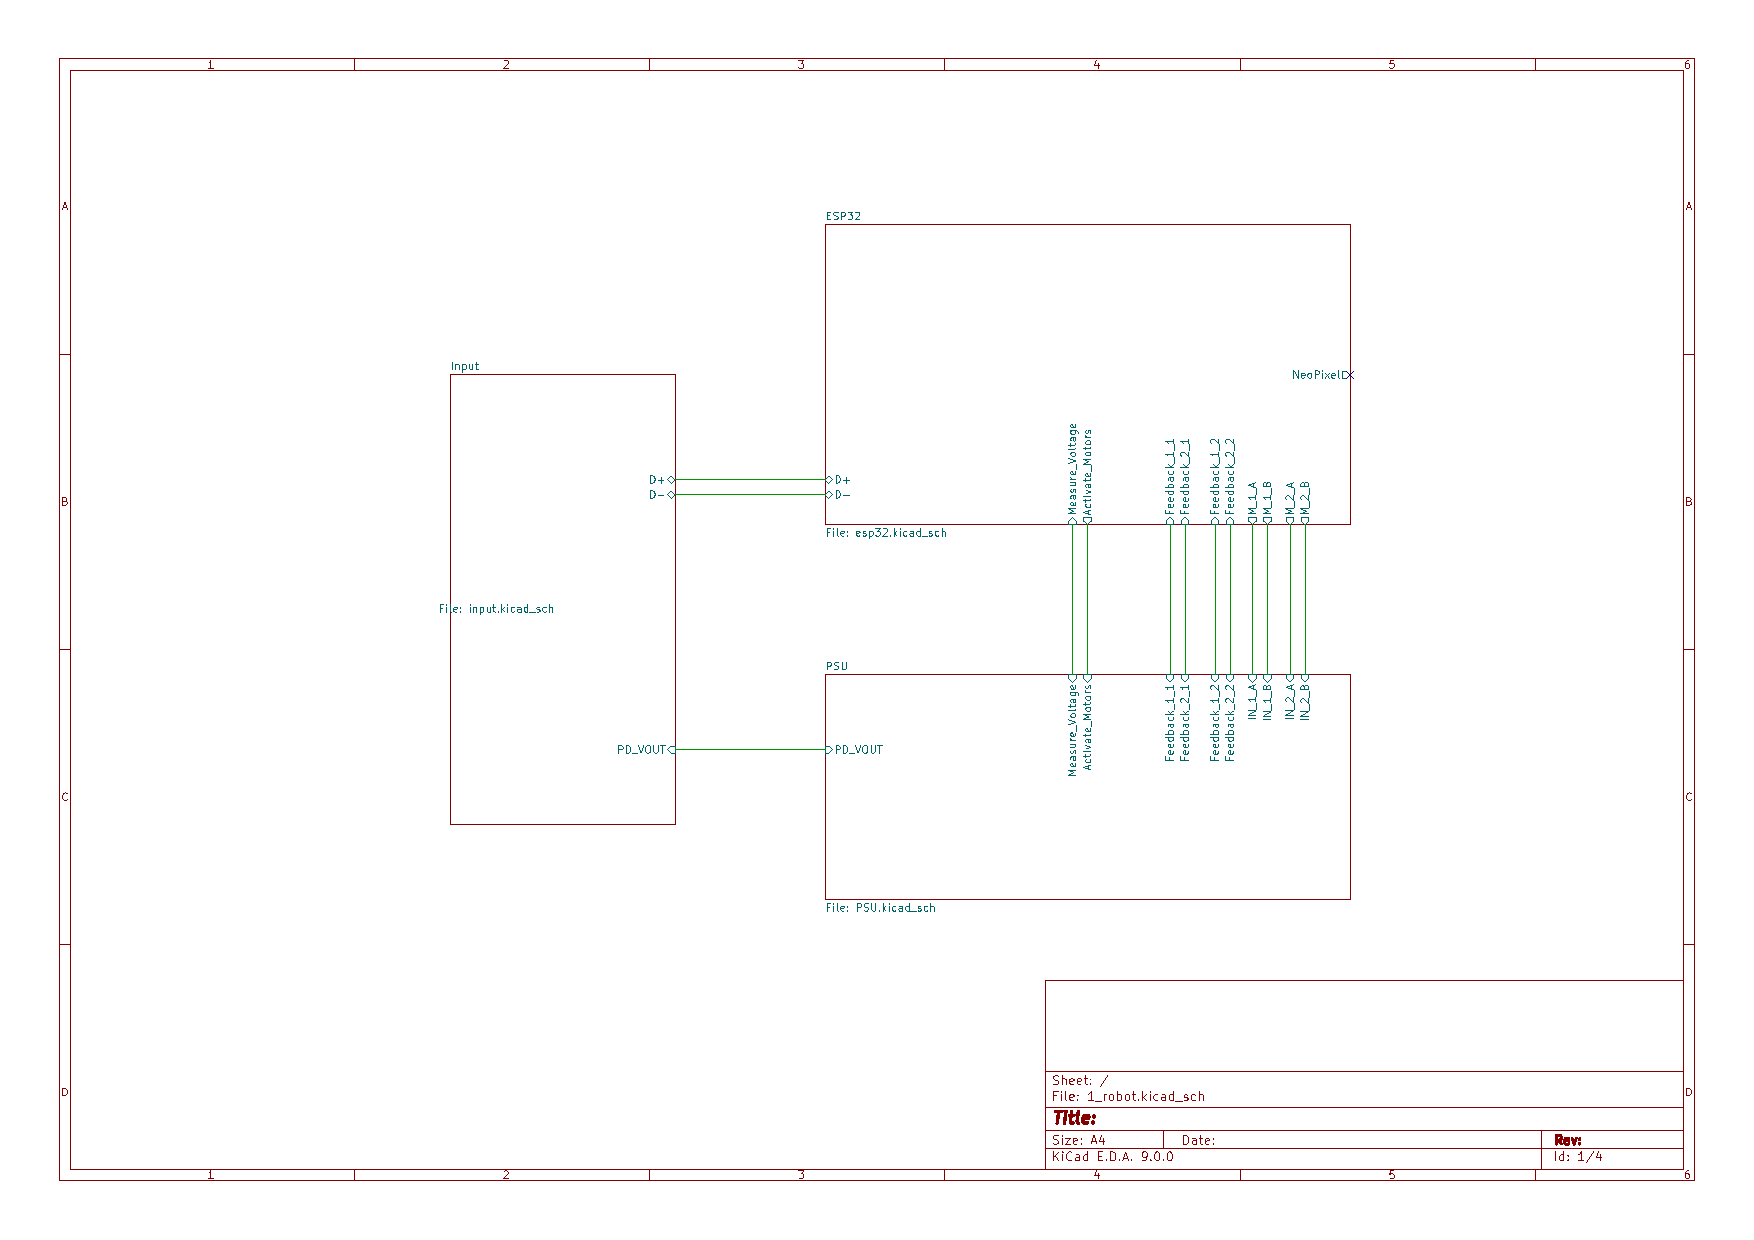
\includepdf[angle = -90]{obrazky/1_robot.pdf}

\subsection{Vstupy}
Byl odstraněn převodník USB na UART, jelikož ESP32 S3 má zabudovaný interní.
\newpage
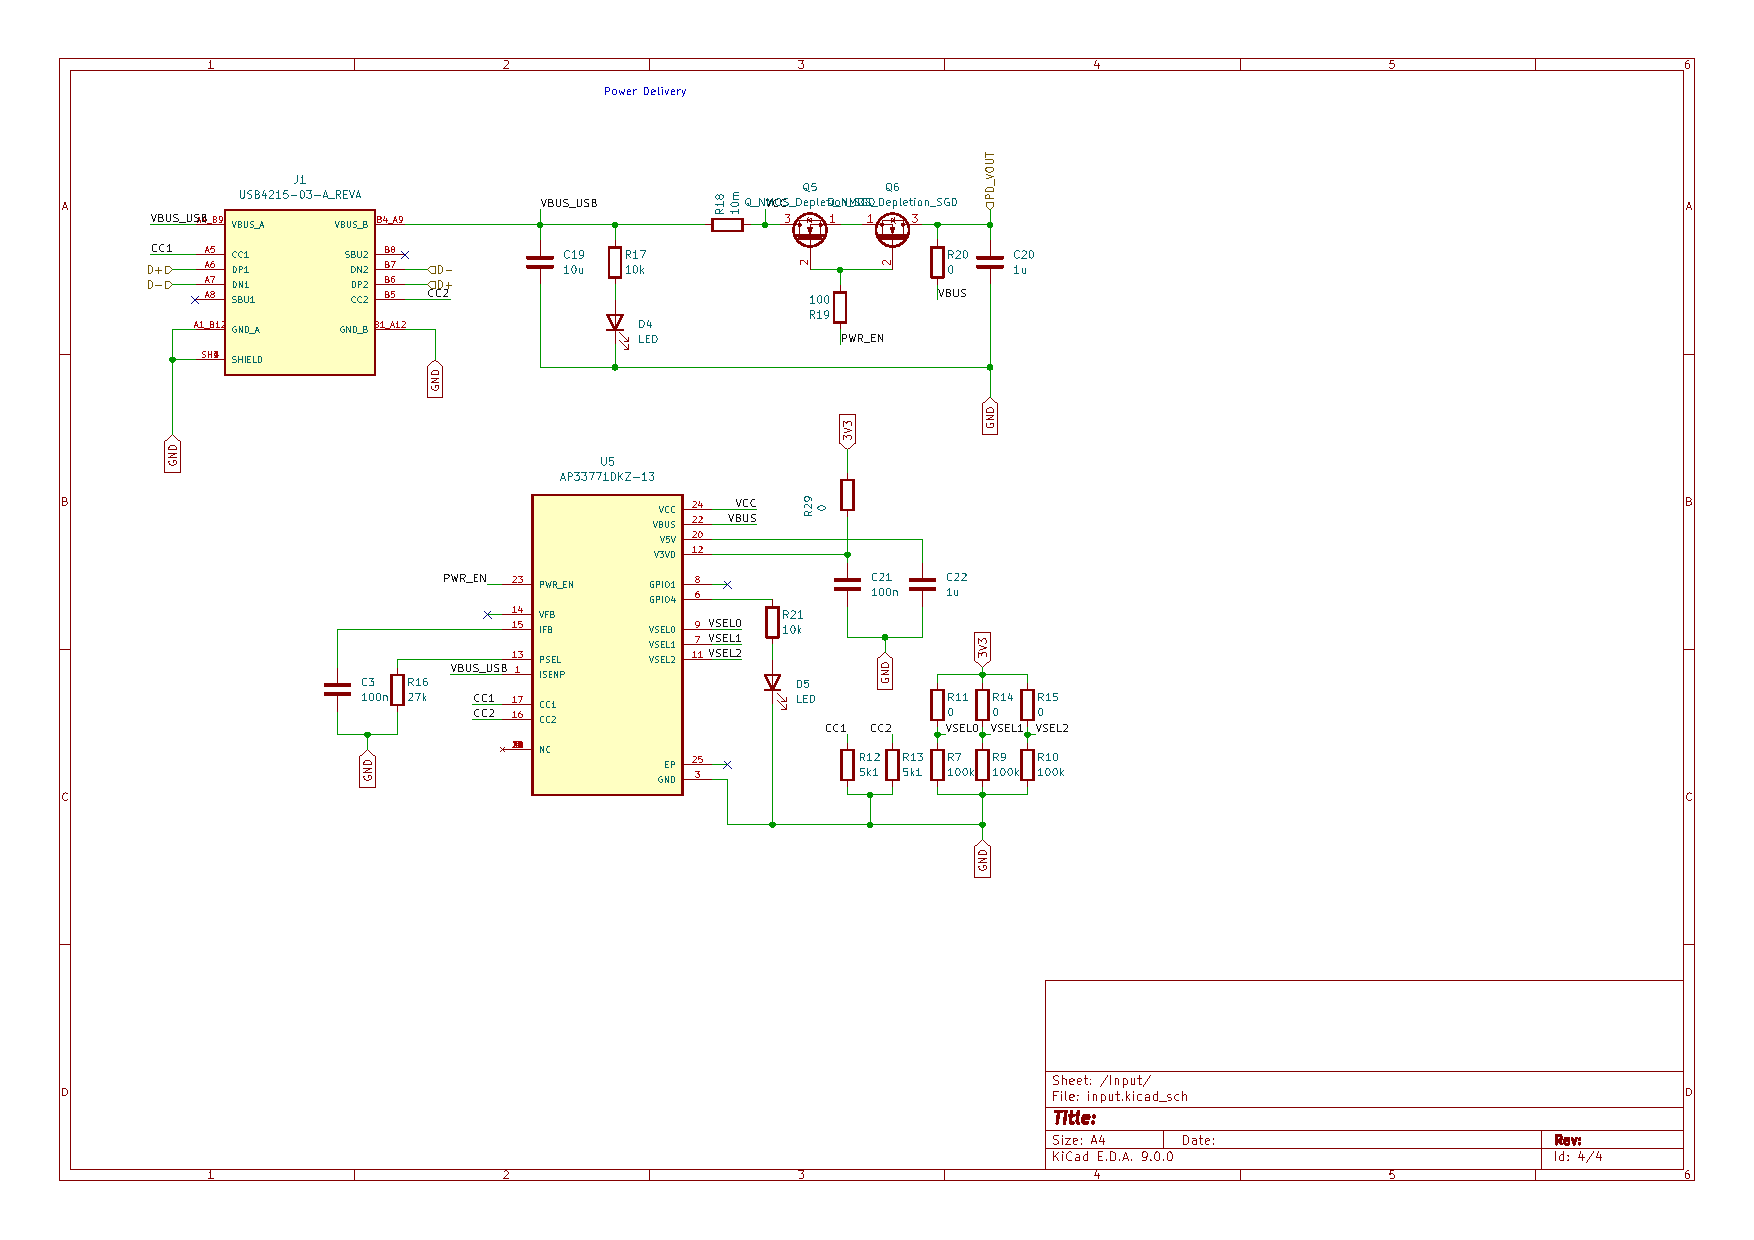
\includepdf[angle = -90]{obrazky/1_robot-Input.pdf}
\subsection{ESP}
Pro SD kartu byly přidány PULL-UP rezistory. Pro přepnutí SD karty do režimu SPI jsou tyto rezistory povinné.\\
Dále přidám modul MPU6050, kdyby BMI160 nefungoval, ať existuje jistá záloha.\\
USB připojeno přes $0 \Omega$ rezistory pro případ, kdyby byly s USB problémy.\\
Část schématu pro STRAP piny byla uhlazena a reozganizována.\\
Veškeré piny ESP32 jsou vyvedeny na externí konektory.


\newpage
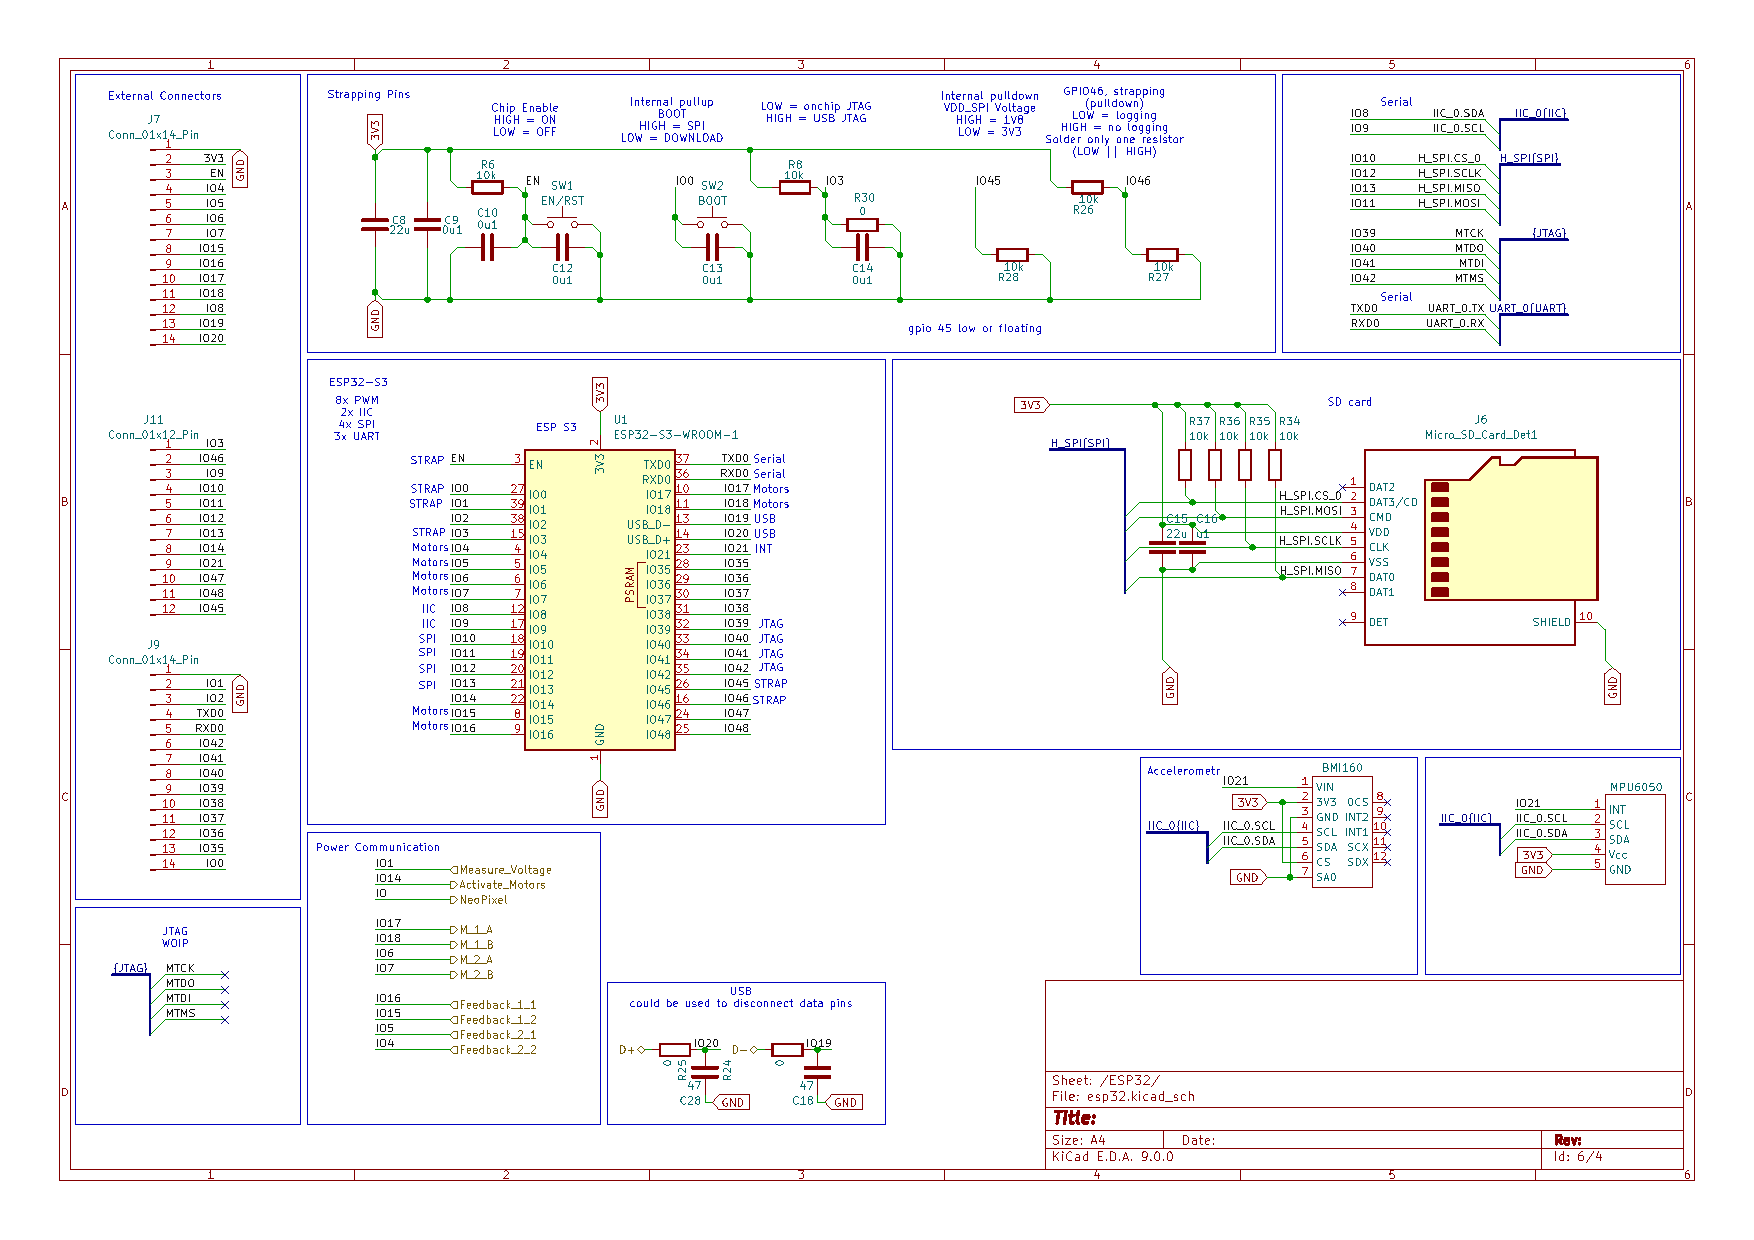
\includepdf[angle = -90]{obrazky/1_robot-ESP32.pdf}
\subsection{Napájení}
Největší změnou je absence napájecího obvodu. Na podnět oponenta práce "Proč nevyužiješ rovnou PD čip?" Jelikož lze napětí Power Delivey omezit na 8.6V, což je napětí dvou nabitých článků 18650, a omezení napájecího výkonu na 18W, což je napájecí proud okolo 2.5A, by s tímto řešením neměl být žádný problém. V případě nefunčnosti lze odpájet $0 \Omega$ rezistor a fungovat pouze na externí nabíječku článků.\\
Další změnou je použítí jiných H můstků. Byly zvoleny můstky s vyšším maximálním zatížením a vyšším napětím.


\newpage
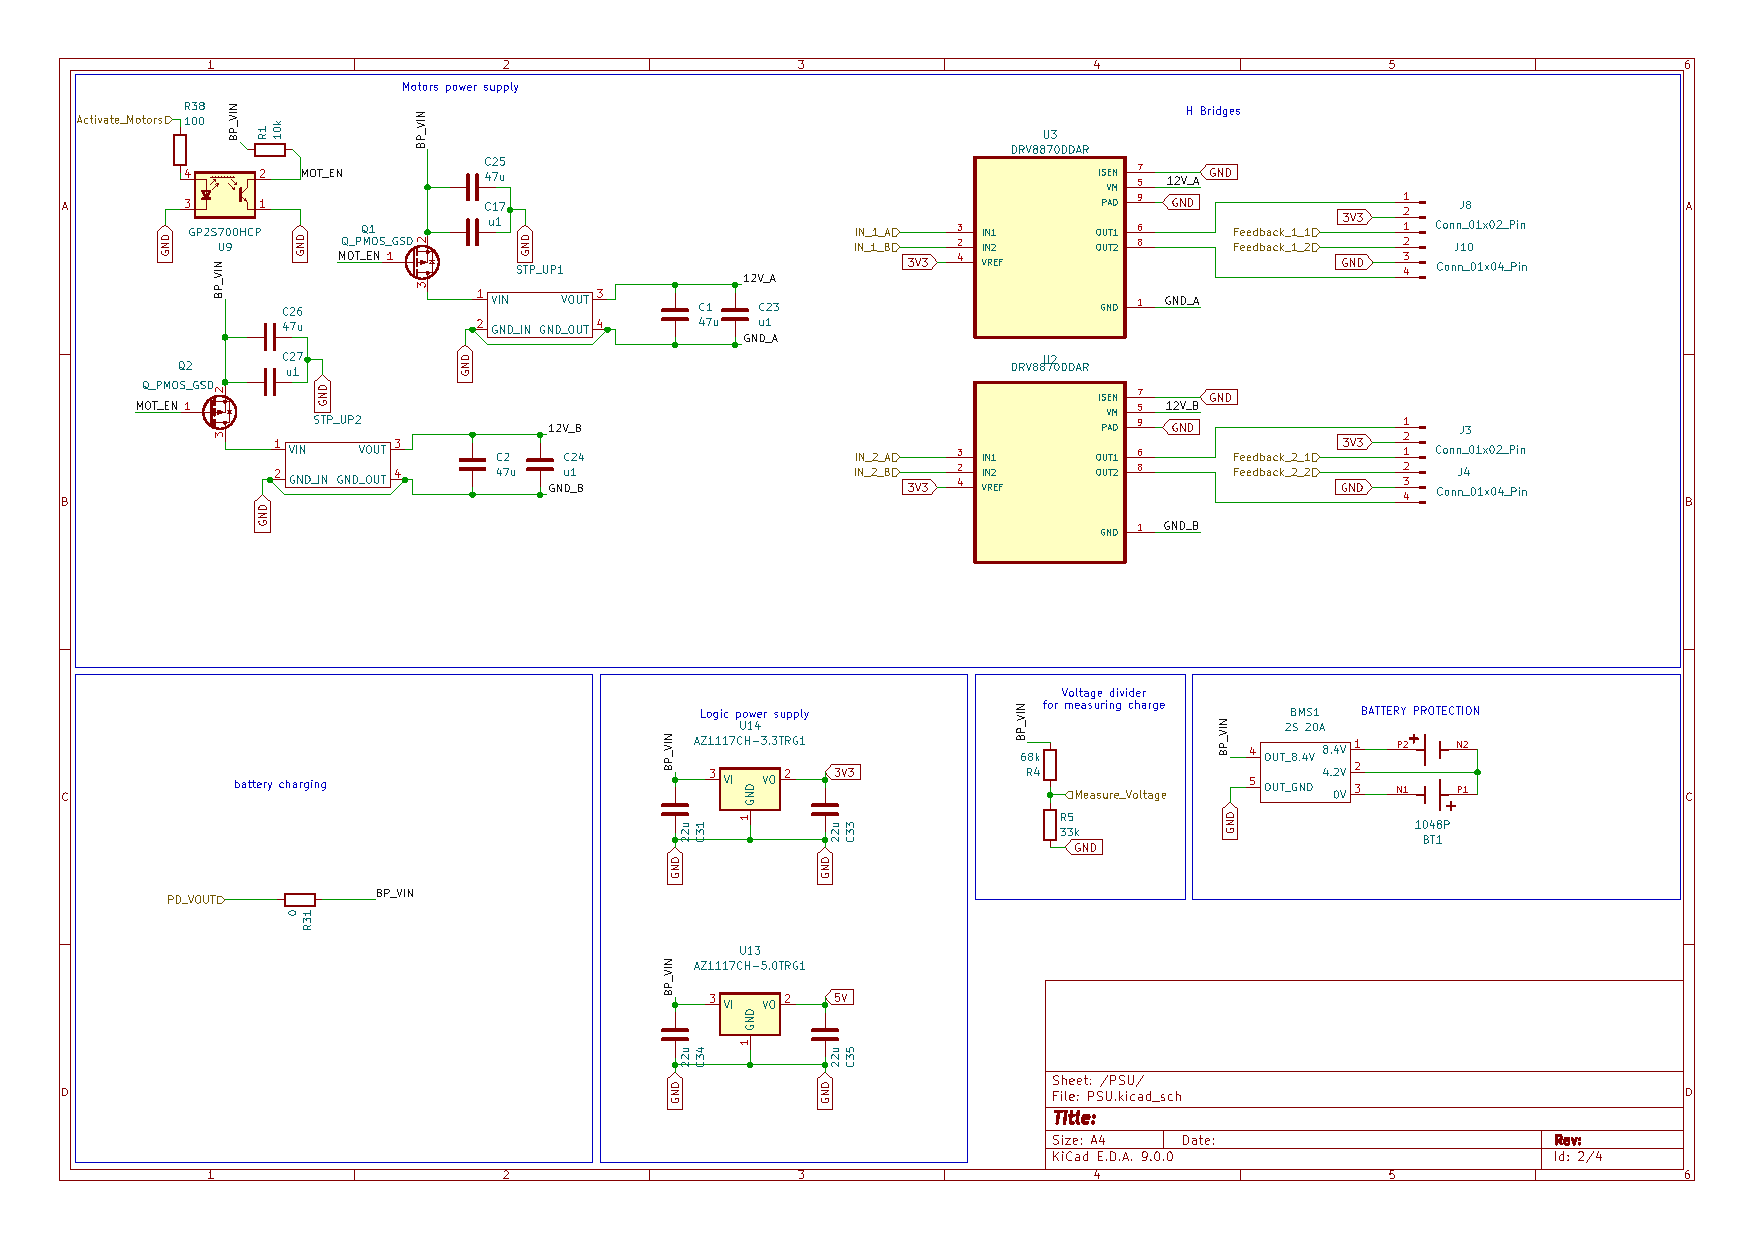
\includepdf[angle = -90]{obrazky/1_robot-PSU.pdf}




